\chapter{Architectural and Design Decisions}
In this chapter, we look over the design decisions that influenced the shape of the library along with a theoretical comparison of various models or architecture, pointing out advantages and possible use cases for each of them. The purpose of such a section is to justify the way the framework is intended to be used as well as pointing out the differences in relation to other popular ways of achieving a similar result.

\section{Design Principles}
Understanding the design principals on which a framework was build is a key part of quantifying if the desired result was achieved whilst guiding the development process in the right direction.
While many of them seem rudimentary or obvious, many others were left out, such as cross-platform compatibility, design for failing, or crash stability. Some of the design decisions are presented below, along with some reasoning behind them below, in order of importance.

\begin{enumerate}
\item \textbf{Speed} Speed is one of the most important factors we look after. In order for the framework to be speed-reliable, it should do a decent number of "ping-pong" (a→b→a→b…) operations per second, i.e., having 2 services that talk to each other as much as they can to share some meaningful information or to simulate an actor. As a decent benchmark for this, for the majority of the cases, $10^6$ operations per second seems a decent enough number to strike for. 

\item \textbf{Ease of use and reducing glue code} Being able to write code without having to copy-paster or follow a lot of generic code is a must. The most important thing is to be able to get something done with at little code as possible while maintaining a generic enough API. Glue code and heavy APIs represent an important source of bugs. Forcing developers to write meaningless code decreases the overall attention to details, letting subtle bugs to be created in the weirdest scenarios.

\item \textbf{Fast scaling} While scaling is an important factor and advantage in microservice-based applications, the speed scaling speed becomes an important factor to look after. The rise of AWS (Amazon Web Services) allowed new tools to be popularised in the DevOps(software development - Dev and information-technology operations - Ops) community such as elastic scaling. This allows for automatic deployment in case of a sudden increase in requests. Pandora.cc tries to take this a step forward, enabling a fast repurposing and reorganization of the structure of the project without any required downtime.

\item \textbf{Easy Deployment and Upgradeability} Being able to perform easy deploy operations is an important aspect of developing, especially if deployment is involved in the testing process. Sometimes seen as a new deployment, being able to upgrade current services that are already deployed is possible with Pandora.cc. In order to achieve this, some specifications needed to be set beforehand. We chose to opt to be able to change individual implementations of nanoservices while the Pandora binary is still running, the only downside being the need to upgrade all implementations, in case there are more running instances of such service, along with a loss in state for the specific services. Still, it's possible to implement cold storage caching, which will mitigate such cases.

\item \textbf{System design optimizations} Synchronization is seen as one of the biggest pitfalls in parallel programming. We try to allow developers to reduce the number of synchronization mechanisms required by giving more access to the underlying hardware. By individually specifying each nanoservice on which CPU-core it should run, 2 specific nanoservices could be forced to not run in parallel by forcing them only to be scheduled on a specific CPU. Another aspect to this is the fact that if the configuration is done right, a specific nanoserviced could be the only one being scheduled on a CPU-core, thus allowing for dedicated threads for latency-sensitive services, which should be available as soon as possible, without waiting for something to finish before they could start.

\item \textbf{Reducing bugs} Programming languages are not equal. Some of them are associated with more bugs, such as C, C++ or Python while others are not, such as Haskell, Scala or Clojure\cite{progimpact}.

 While C++ is naturally associated with more bugs, developing in a specific way using a well-thought library can greatly reduce the number of bugs due to reducing some of the usual bug causes. The goal is to reduce such practices, such as race-conditions and the usage of pointers, explicitly the tracking of ownership. We try to achieve this by enforcing the use of nanoservices, which force the writing of code in such a way that the data needs to be shared less around scopes, making it easier to keep track of and by offering another toolset to go around synchronization mechanisms.
\end{enumerate}

\section*{Position relative to the state of the art}
Instead of trying to implement an architecture based on the textbook definition, Pandora.cc tries to blend in ideas from various technologies in order to succeed in a particular area of interest. The main reason for this lies in the current state of the art: there are well-established frameworks that implement the microservice architecture (Google C++ RPC or POCO) for C++ and various other alternatives for different languages. 

In order to make the framework worthwhile, some really important advantages needed to be added for specialized use-cases so that the advantages would overcome the cost of adding or switching to a new paradigm. Taking this into consideration, we'll evaluate 3 main technologies, namely microservices, nanoservices, and the actor model, with the intent to create a new blend that will fulfill the design principles.


\section{Microservices}
Even thou the concepts used by microservices were used before by SOA, a better definition of the paradigm in 2013 led to a rise in popularity in the following years\cite{klock}. Since the technology is relatively new and can be implemented differently, we chose to refer to \cite{viggiato} as a baseline on how the industry adopted and used this paradigm as well as finding out where the advantages and challenges are situated in contrast to the literature.

\subsection*{Advantages}
\begin{itemize}
\item \textbf{Independent deployment} allows teams to upgrade the system as they roll out new features and bug fixes \cite{newman}, the main beneficiary from this being the user, which gets the new and latest as fast as possible. This enables teams to be more independent from each other, thus reducing bureaucracy inside a company and allowing for faster development overall. 
\item \textbf{Scalability} is often mentioned as one of the main advantages, especially over monolithic architectures \cite{alshuqayran}. Due to the distributed design, microservices allow the scaling of one specific service instead of scaling the whole system.
Maintainability is achieved due to the design of the communication pipeline, each microservice implementing a stable API while having RPC (Remote Procedure Calls) over the internet as the means of sharing or requesting information.
\item \textbf{Language independence} is the staple of distributed programming. The use of REST API or cross-language serialized data structures such as Google's Protocol Buffers made microservices language agnostic for the most part, enabling a wide range of developers to be able to contribute to a shared codebase.
\item \textbf{Easy deployability} is not necessary a microservice advantage per se, but more a result of the DevOps practices which are used when working the technology. The rise of containers such as Docker and the wide coverage for such technologies by server providers allow the deployment of microservices into Docker containers with ease, which can afterward be deployed in the cloud. This is possible due to the general aspect of docker containers and encapsulation of resources in the container itself. 
\end{itemize}

\subsection*{Disadvantages and challenges}
\begin{itemize}
\item \textbf{Expensive RPC} due to the overhead of the network involved in each operation can quickly add to a large overhead, especially in complex queries that require sequenced RPC to yield the final result\cite{viggiato}.
\item \textbf{Service faults} tend to be harder to debug or to track the origin of the problem due to the distributed aspect of microservices\cite{viggiato}. Maybe one of the biggest disadvantages compared to the monolithic architecture, miss behavior tends to be harder to identify, especially if the error is introduced in the runtime of another service than the one that crashed. This becomes even harder if that service is written in another language.
\item \textbf{Testing} a stack of services can be challenging, especially due to random events that could occur in a normal deployment, such as network errors, DB bottlenecks, or random crashes\cite{viggiato}.
\item \textbf{The complexity of distributed systems} is no easy task, access to data or data synchronization being one of the major problems\cite{viggiato}.
\end{itemize}

\subsection*{Other important characteristics}
In the majority of cases and implementations, microservices are accompanied by some characteristics such as being autonomous components that run on one process\cite{hassan}. This is specifically important since it enables them to self-heal in case of a system failure due to limited scoping, which so the failure doesn't affect other systems and redundancy to replace the failed service.

\subsection*{Applications}
Monzo is a digital bank(neobank) startup based in London, UK, which has a user growth of 40'000/week\cite{monzo}. It was founded in 2015, and it has a transparent policy regarding its development practices. This is why we chose to showcase some of their findings, as they reflect state of the art in terms of development practices.

\begin{figure}[H]
\centering
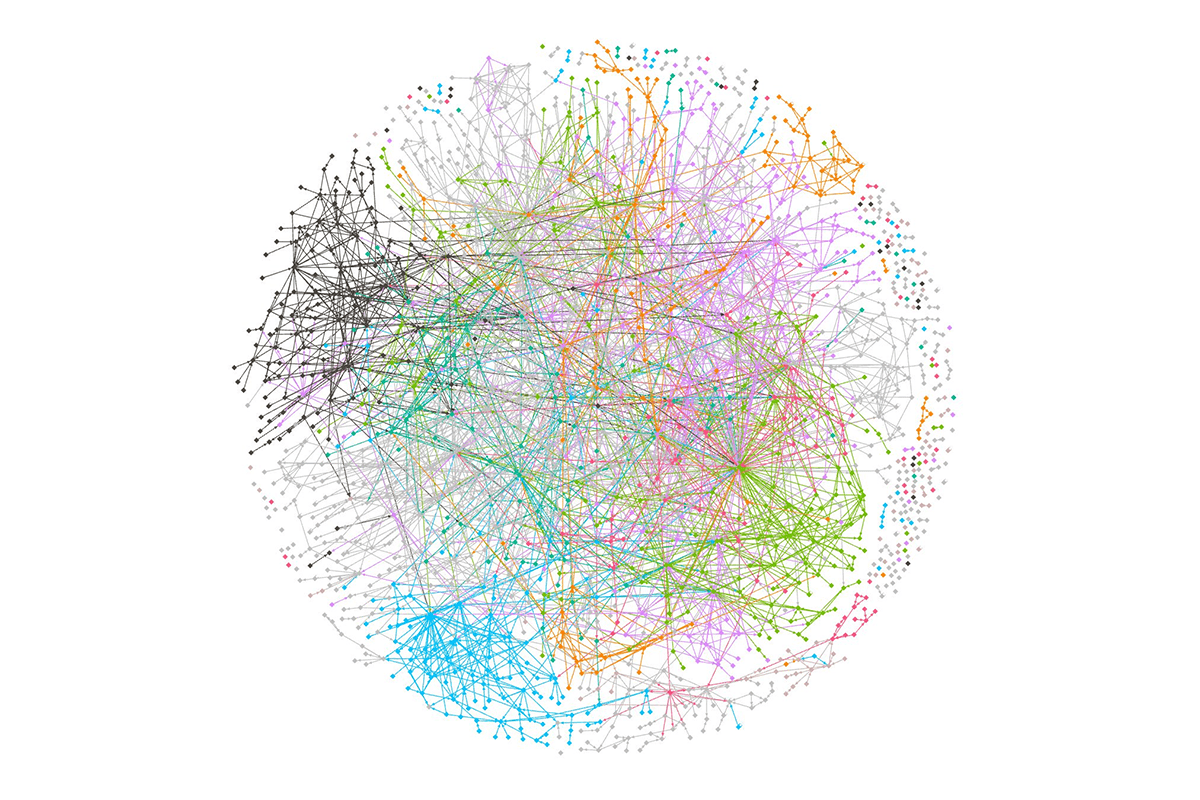
\includegraphics[width=1\linewidth]{content/fig/monzo-microservices-team-colored.png}
\caption{Monzo's microservices map}
\end{figure}

Figure 4.1\cite{monzo}, showcases the architecture of the digital bank, each node in the graph representing a service and one edge showcasing an enforced network rule between them. The nodes are colored based on the team that manages them. 

The purpose of the figure is not to start a debate on whatever or not the company uses the architecture right, but to showcase that it's possible to achieve tremendous scaling compared to other architectures due to the widespread solutions to facilitate this, such as Kubernetes.

More details regarding their findings can be found in other blog posts as well, such as 'building a modern backend' which dates back in 2016, one year after the company's launch.
Without going into detail, Monzo's findings are similar to the ones presented above\cite{viggiato}.

\subsection*{Breakdown}
The majority of the advantages and disadvantages of microservices have their root in remote calls. This enables services to be independent of each other while being harder to test and design. To allow a better deployment and failure handling, each microservice is seen as a separate entity, being independent of other components.

\subsection*{Takes}
While microservices offer a great way to design full-scale applications, they lack in speed and usability for small applications or applications that did not meet the required necessity for such infrastructure yet. We argue that it's a big decision to be made, one that pays off in the big run, but it will surely not favor such practices to be adopted from the beginning. On the other hand, a later transition to this pattern requires a massive change in code-paradigm, which could take much time to be integrated. 

The containerization of microservices is a widely used and implemented feature, but we feel it shouldn't be enforced. By allowing multiple microservices to be run in the same process, we can cut off the RPC induced latency completely, thus making the architecture a viable option for both vertical and horizontal scaling. By doing so, some advantages become harder to achieve, like easy deployability, independent deployment, and crash robustness. We try to offer a good workaround for the first two using Pandora.cc specific tools like the bundling system and the hot-swap service. These tools are explained in more detail in chapter 4.7.

\section{Nanoservices}
With the rise in popularity of microservices in 2014, people started talking about taking the paradigm a step forward. Microservices were seen as a smaller approach to SOA, while nanoservices were defined as a smaller microservice, ranging from 10 to 100 lines of code. It took 4 years until developers figured out a way to make this technology reliable. The rise of nanoservices was made possible due to the maturity of the microservices ecosystem and the parallel rise serverless, a new technology that tries to tackle the same problems. These changes didn’t solve the disadvantages of nanoservices, but instead, it offered a different point of view to consider when considering to build a nanoservice.

\subsection*{Advantages}
\begin{itemize}
\item \textbf{Deployability} is taken a step forward compared to microservices, nanoservices also containing all the required infrastructure necessary to be deployed. The definition of such service also handles all resources required during its lifetime. To integrate the service in the ecosystem, a config file is used to specify different parameters of endpoints for events.
\item \textbf{Reusability} is a significant advantage due to the limited scope and ease of integration. This is highly enhanced by the fact that nanoservices can be coded in any language, and they can be bundled into a Docker container. Due to this nature, a “Microservice Package Manager” could be more significant than any language-specific package manager, such as pip for python and npm for javascript.
\item \textbf{Usability} is often showcased as an essential advantage. Nanoservices should do something or figure solve a problem, meaning that they are not to be used inside a complex chain and should be mostly situated at the end of the execution chain.
\end{itemize}

\subsection*{Disadvantages and challenges}
\begin{itemize}
\item \textbf{“Nanoservice pattern is an anti-pattern”} is often used to describe nanoservices in relationship to microservices. Being more of a pitfall, building entire services around nanoservices could escalate quickly into unreliable code and an increase of complexity in deployment.

\item \textbf{Communication overhead} is accentuated compared to microservices since nanoservices produce more remote calls due to the limited scope. This makes SLAs (service-level agreement) challenging to reason about since many interrupts can happen in the life-cycle of a request inside a nanoservice-based architecture.
\end{itemize}

\subsection*{Breakdown}
Nanoservices occupy the role of containerized, scalable, and language-agnostic endpoints to different services, such as databases, storage units, or cache managers. Tooling is a common use-case for nanoservices, such as cost managers for cloud computing, alert systems, or data aggregators.

\subsection*{Takes}
Nanoservices can be used in the majority of cases to take care of communicating with an endpoint or adding plugins to an application. We argue that by moving the nanoservices closer to the microservice, we can reduce the network overhead, raising the potential of such nanoservices. This enables nanoservices to be used as a computational part for the request, being a viable option to speed up specific independent tasks, taking a similar role to actors or tasks.


\section{Actor model}
Introduced by Hewitt et al, the actor model offers a scalable way to implement concurrent software using a 'share-nothing' paradigm\cite{hewitt}. We chose to explore this alternative due to its powerful claims and reduced use case (1), being implemented in Erlang, and various frameworks like Akka, which can be used in both Java and Scala. A new C++ implementation is offered by CAF (C++ Actor Framework) along with with paper\cite{charousset}.

We try to justify the case for (1) reasoning that the performance advantages aligns well with the intended design goals. We base our performance and advantages on the CAF paper while looking at the current state of the art to find systems that use the actor model, focusing on the impact of such cases.

\subsection*{Advantages}
\begin{itemize}
\item \textbf{No synchronization required.} Actors do not share stare and achieve sharing data by passing messages. The lack of synchronization mechanisms enables less error-prone code due to race conditions.
\item \textbf{Small memory footprint.} Actors are lightweight units of computation, each of them taking less then 0.5KBs of memory, including the associated mailbox. This enables the creation of $2^{20}$ actors in less than 10 seconds, having a memory footprint less than 500MB\cite{charousset}.
\item \textbf{Fast communication for same-machine use cases.} A proper implementation of the mailbox can achieve performant results such as $20 \times 10^6$ messages being sent and processed by one actor in a $20:1$ scenario, in under 10 seconds.\cite{charousset}
\item \textbf{Fault tolerance.} Each actor can crash independently without affecting the whole system, such cases being handled by a supervisor, another actor who decides how to handle the event. \cite{hewitt}
\end{itemize}

\subsection*{Disadvantages and challenges}
\begin{itemize}
\item \textbf{Immutability} is not necessarily a disadvantage, but it's most common in functional programming. This inherently makes developers adhere to a new programming paradigm, thus increasing the complexity of designing and writing code.
\item \textbf{Dining philosophers problem} is often presented as one of the pitfalls of the actor model. The no synchronization paradigm creates a different range of problems that require different solutions. Similar to the immutability challenge, this imposes a different mindset than the general development process of parallel programming.
\end{itemize}

\subsection*{Breakdown}
The actor model proposes a fast and reliable paradigm that best suits functional programming since it'll blend in with the fact that such languages do not use mutable variables and focus more on keeping a consistent state throughout the run of the service. While CAF offers a good API and competitive performance, we argue that the development process is to different from being considered as a viable option for an application.

\subsection*{Takes}
The majority of the challenges that come with the actor model are related to the development process, and we argue that there are good partial-use cases to justify the case for the actor model. While applications that use only the actor-model are too demanding, using this practice for maintaining state is often the everyday practical use. For example, an online shop might choose to have one actor for each item sold in its store.

While the actor model does not fulfill the entire design principles, it offers a useful benchmark when taking into consideration speed and, in some ways, scaling.


\section{Conclusions}
All the architectures described in the section provide valuable advantages while having their disadvantages or posing difficult challenges. We acknowledge that other design patterns may solve some of the problems or provide suitable alternatives to the proposed ones, but we consider that this selection provides a right mix of options while keeping the selection base clean enough.

Considering all these, we designed Pandora.cc to offer a similar performance to the Actor Model while allowing a development style similar to the nanoservice architecture, all while having the deployment and scalability capabilities of the microservice architecture.

We argue that the Actor Model is an excellent paradigm if implemented in a functional language, but when used in an imperative language like C++, it lacks powerful tools that enable the immutability aspect of actors. This is solved by changing the actors with nanoservices. 

Nanoservices can be used in a great variety of use cases due to their general aspect and easy reusability. While the communication and deployment overhead is considered as being too much when used in an application, we try to repurpose them by filling the role of an actor. This reduces the communication overhead dramatically while maintaining all the functional aspects of nanoservices.

Microservices appeared first as a loosely defined term to refer to a more granular Software Oriented Architecture. In time, it became more mature due to the support from big tech companies, which benefited the most from the approach, allowing them to scale in a way to match the unprecedented growth. This enabled the microservice architecture to be implemented, deployed, and tested with ease due to the number of popular DevOps tools, such as Kubernetes, Docker and Jenkins. We argue that this architectural style was a success due to the abundance of tools, and such we try to allow Pandora.cc developers to take full advantage of them, by creating ‘microservices’ as bundles of nanoservices, like a plug-in system. This approach is made using the bundling system, a powerful tool that will be showcased in chapter 4.6.

\subsection*{Tradeoffs}
\begin{itemize}
\item Since 3 different coding paradigms inspire Pandora.cc, the resulting features are not a union of the original ones. Some of them are diminished while some disadvantages are less severe.
\item Since Pandora.cc is a C++ framework, microservice’s language independence does not apply when developing with Pandora, compared with Google’s RPC, which supports out of the box cross-language endpoints for different services. Services written in different languages can be supported, but a pandora-specific mockup service interface needs to be created.
\item Nanoservices reusability is diminished since they need to be Pandora nanoservices. We still think it’s easy to port C++ nanoservices wrote using other frameworks to be Pandora-compatible, but this won’t come out of the box. The actor Model’s fault tolerance is wholly negated due to the introduction of nanoservices instead of actors. Nanoservices alone are fault-tolerant, but when running inside the same process, a big fail can affect other nanoservices as well.
\end{itemize}

\section{Tools}
To make Pandora a competitive alternative, we created a series of tools to consolidate development practices. They are not inspired directly from any paradigm but instead developed to tackle some problems.

\textbf{Bundling system.} Since Pandora.cc organizes a project as a collection of nanoservices, the bundling system allows the creation of bundles, providing a level of abstraction while making the deployment and management process more straightforward. For example, one bundle could be called FileMicroservice, which would contain the FetchFile, WriteFile and DeleteFile nanoservices. The FileMicroservice can be used in the future as a single entity without worrying about future changes in the structure of the microservice, such as the inclusion of new nanoservices or changes in API.

\textbf{Thread selection} can be a powerful tool that if used correctly, but it can be tough to design applications this way. It allows both enforcing of restrictions to avoid race conditions as well as allocating resources for a service so it can start serving as fast as possible. To make the development more accessible, we chose to not enforce this, as it can be hard to catch potential bugs, but it allows for more control over the runtime of the system.

\textbf{Nanoservice hot update.} Since nanoservices are embedded in the executable, the naive way would be static link them into the binary. Instead, Pandora builds each nanoservice as a dynamic library that can load at runtime, allowing the libraries to be unloaded and reloaded, thus allowing updating the DLLs while the binary is running. 